\documentclass[12pt]{article}
\usepackage[utf8]{inputenc}
\usepackage[a4paper,left=4.5cm,right=1cm,top=2.5cm,bottom=2cm]{geometry}
\usepackage[onehalfspacing]{setspace}
\usepackage{graphicx}
\usepackage[ngerman]{babel}
\usepackage[T1]{fontenc}
\usepackage{microtype}
\usepackage{hyphenat}
\usepackage{url}
\usepackage{booktabs}
\usepackage{tabularx}
\usepackage{bibgerm}

\newcommand*{\quelle}{% 
  \footnotesize Quelle: 
} 

\title{Intelligenter Labyrinth-Roboter}
\parindent0pt

\begin{document}
\newgeometry{
  left=3cm,
  right=3cm,
  top=2.5cm,
  bottom=2cm,
  bindingoffset=5mm
}
\begin{titlepage}
	\centering
	
\includegraphics[width=0.15\textwidth]{sg-logo.png}\par\vspace{1cm}
	{\scshape\LARGE Söderblom Gymnasium \par}
	\vspace{1cm}
	{\scshape\Large Projektdokumentation\par}
	\vspace{1.5cm}
	{\huge\bfseries Intelligenter Labyrinth-Roboter\par}
	\vspace{1.5cm}
	{\Large Jan Beckschewe und Jan Reimer \par}
	\vspace{1.5cm}
	Fachlehrer: Herr Salloch \par
    \vspace{0.5cm}
    Verfasser: Jan Reimer \par
    \vspace{1cm}
	Schuljahr 2016/17 \par
    
	\vfill

	{\large \today\par}
\end{titlepage}
\restoregeometry
\tableofcontents
\thispagestyle{empty}
\newpage
\setcounter{page}{3}
\section{Einleitung}
\paragraph{Allgemein} Robotik ist ein Feld mit vielen Anwendungsmöglichkeiten. Von Militärrobotern bis zu Robotern die Menschen aus Trümmern helfen, aber auch bei gewöhnlichen Dingen wie im Haushalt spielt die Robotik eine immer größer werdende Rolle. Viele Menschen sind an Robotik interessiert, jedoch gibt es Probleme die im Weg stehen: ungeeignete Umgebung und ungenaue Sensoren erschweren den Einsatz erheblich.  

Das Labyrinth besteht aus dünnem schwarzen Klebeband das auf einer weißen Tapete angebracht ist. Um das problemlose abfahren des Labyrinths zu ermöglichen müssen mehere Faktoren beachtet werden: Bewegungskontrolle in Kombination mit Sensorik, Lösungsalgorithmen für das Labyrinth sowie das Design des Fahrzeugs.

\paragraph{Zielsetzung} Unser Ziel war es einen intelligenten, kleinen und autonomen Roboter zu bauen der ein beliebiges Labyrinth lösen kann in dem er den kürzesten/schnellsten weg zum Ziel findet. Diese Dokumentation wird die notwendige Hardware erklären, angefangen mit dem Mikrokontroller bis zur Auswahl des Akkus. Zusätzlich werden verbreitete Lösungsalgorithmen für Irrgärten auf ihre Tauglichkeit für unser Projekt überprüft. 

\paragraph{Was ist ein Microcontroller?} Ein Mikrocontroller ist ein kleiner Computer in einem einzigen Integrierten Schaltkreis (englisch integrated circuit, kurz IC). In der modernen Fachsprache werden Microcontroller als 'system on a chip', Ein-Chip-System oder auch kurz als SoC bezeichnet. Ein Microcontroller beinhaltet einen oder mehrere CPUs (Prozessoren) sowie Speicher und programmierbare I/O Schnittstellen. Außerdem ist oft Programmspeicher, RAM und komplexe Peripherie wie USB- (Universal Serial Bus), I$^2$C- (Inter-Integrated Circuit) Schnittstellen verbaut . Microcontroller sind für den Einsatz in 'embedded applications' (deutsch: eingebettete Systeme) entworfen, im Gegensatz zu Mikroprozessoren die in PCs verwendet werden.

Microcontroller werden in automatisch kontrollierten Geräten wie in Motor\hyp Kontrollsystemen, medizinische Impantaten, Fernbedinungen, Elektrowerkzeug, Spielzeug und in vielen anderen embedded systems benutzt. Die ständige Reduktion der Größe und Kosten von Microcontrollern macht es technisch und wirtschaftlich möglich immer mehr Geräte und Prozesse digital zu steuern. Mixed signal Microcontroller sind weitverbreitet, um analoge Komponenten zu integrieren, das ist notwendig um nicht digitale elektronische Systeme zu steuern.

Manche Microcontroller benutzen lediglich 4-bit Binärwörter und laufen ein sehr geringen Frequenzen um den Stromverbrauch zu senken (einstellige Milliwatt oder Microwatt). Der Stromverbrauch im 'sleep' Zustand (CPU clock und der Großteil der Perheperie ist abgeschaltet) bei wenigen Nanowatt das macht sie perfekt für Anwendungen mit Batteriebetrieb.
\newpage
\section{Theorie}
\subsection{Hardware}
\paragraph{Arduino Uno Rev.3} Der Arduino Uno ist ein Microcontroller Board das auf dem 8-bit ATmega328P basiert er hat 14 digitale I/O pins, 6 analoge Eingänge, eine USB Schnittstelle, einen Stromanschluss, einen ICSP header und einen reset Knopf. Sobald man eine Stromquelle über USB, mit AC zu DC Adapater an die Steckdose  oder einfach mit einer Batterie anschließt kann es los gehen. Man kann sich mit dem Uno austoben ohne viel Angst zu haben etwas falsch zu machen im schlimmsten Fall tauscht man den Chip für wenige Euro aus.

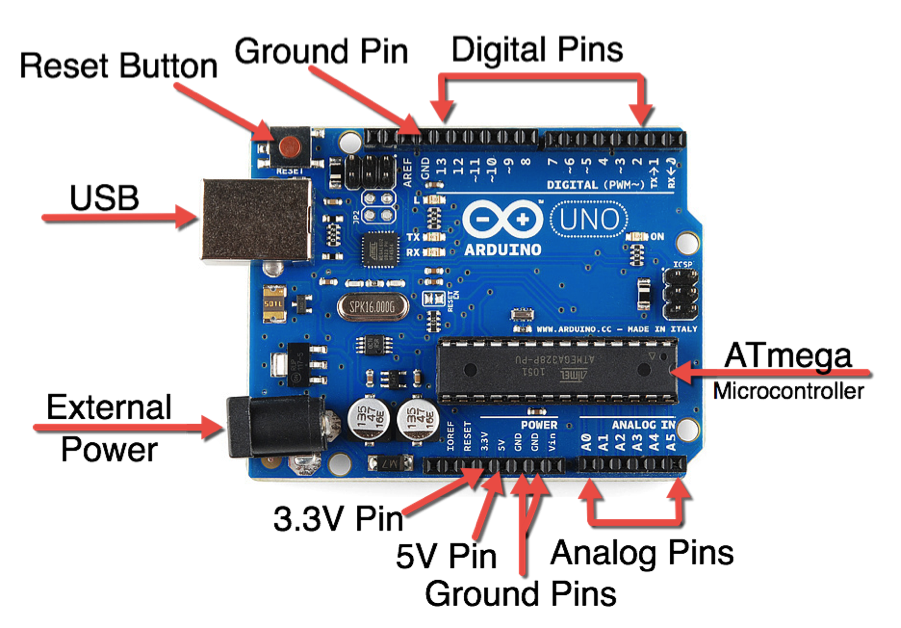
\includegraphics[width=1\textwidth]{ArduinoParts.png}
\quelle\url{https://wiki.eprolabs.com/index.php?title=Arduino_UNO}

\vspace{0.5cm}
\begin{tabularx}{\columnwidth}{XXl}
  Microcontroller&ATmega328p\\
  \hline
  Betriebsspannung&5V\\
  \hline
  Eingangsspannung&6-20V\\
  \hline
  Digitale I/O Pins&14\\
  \hline
  Analoge Eingangs Pins&6\\
  \hline
  DC Strom pro I/O Pin&20 mA\\
  \hline
  DC Strom pro 3.3V Pin&50 mA\\
  \hline
  Flash Memory&32 KB\\
  \hline
  SRAM&2 KB\\
  \hline
  Clock Speed&16 MHz\\
\end{tabularx}
\newpage

\paragraph{Arduino Motor Shield Rev.3} Der Arduino Motor Shield basiert auf dem L298 Dual-Vollbrücken-Motortreiber und ist entworfen um mit induktiven Ladungen umzugehen die beispielsweise von unseren Motoren erzeugt werden. Der Motor Shield ermöglicht es die Geschwindigkeit und Richtung von beiden DC Motoren eigenständig zu regulieren.

\vspace{0.5cm}
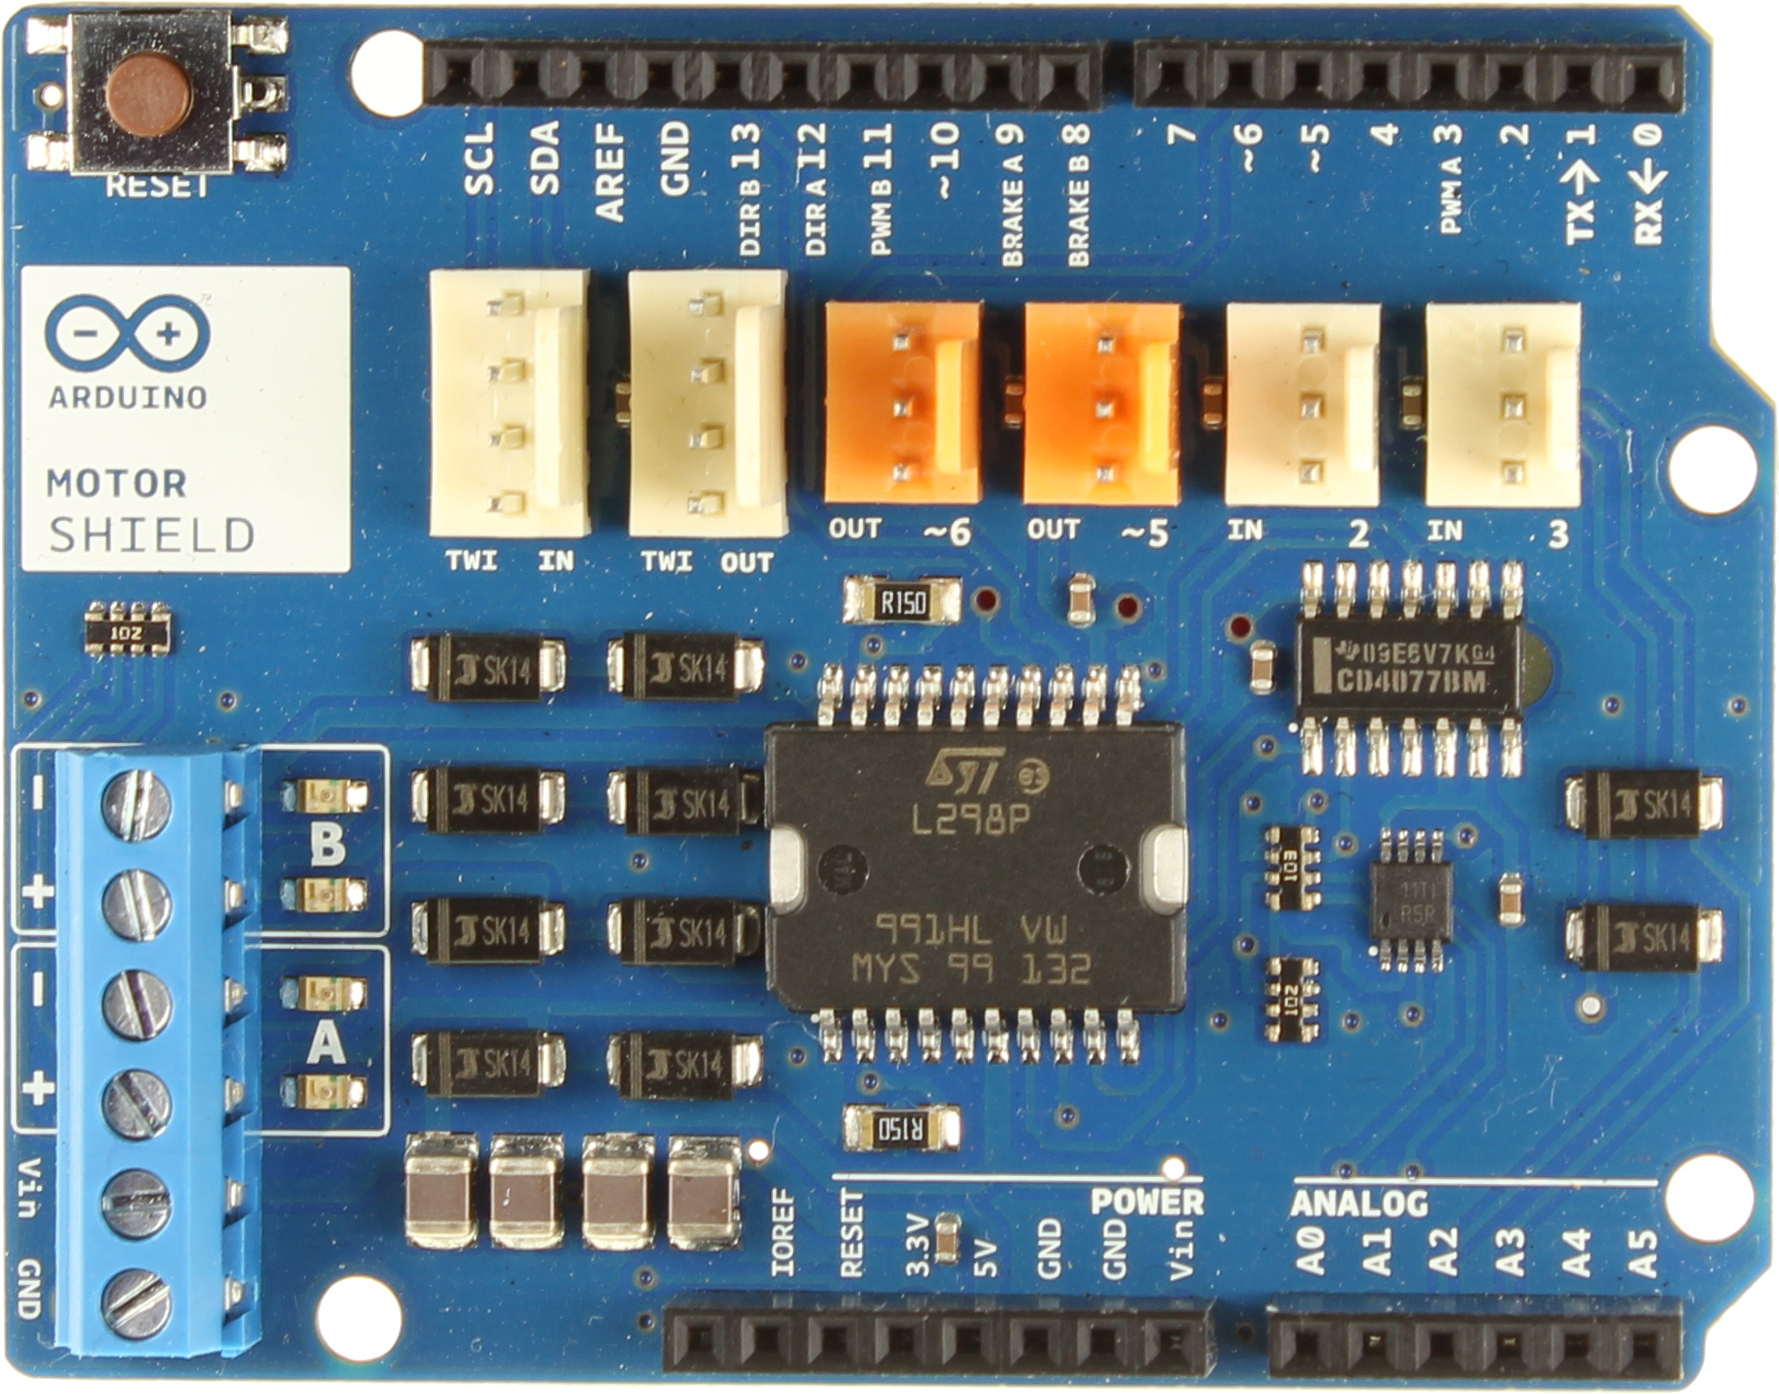
\includegraphics[width=0.7\textwidth]{MotorShield_Front.jpg}\par
\quelle\url{https://www.arduino.cc/de/uploads/Main/MotorShield_R3_Front.jpg.jpg}

\paragraph{Mini Roboter Rover Chassis Kit} Wir haben uns entschieden einen Bausatz zu benutzen um uns das anfängliche Hardware Chaos zu ersparen. Das Kit enthält: 2 Räder, 2 DC Zahnrad Motoren, ein Stützrad, ein Metall Chasis und eine Metallplatte mit Befestigungen.

Da der Aufbau der in der Betriebsanleitung empfohlen ist nicht für unsere Zwecke geeignet ist, haben wir uns entschlossen die Metallplatte an der Unterseite des Autos zu befestigen um die Sensoren möglichst nah an der der Drehachse zu verbauen zudem haben wir das Stützrad weiter vorne angebracht um die Stabilität des Fahrzeugs zu verbessern. Die DC Plastik Zahnrad Motoren sind nicht besonders stark und scheitern am kleinsten Hindernis dennoch sind sie für unsere Einsatzzwecke brauchbar. Das Fahrzeug wird duch eine Powerbank mit Strom versorgt.
\vspace{0.5cm}


\includegraphics[width=0.5\textwidth]{example.png}
\newpage

\paragraph{QTR-8A Reflektions-Sensoren-Array} Der QTR-8A ist zwar als Linien Sensor entworfen und wird auch so von uns genutzt, jedoch kann man ihn auch als Näherungsensor oder auch einfach als Reflektionssensor. Auf dem Modul befinden sich acht Infarotstrahler/Infarotempfänger (Phototransistoren) Paare in gleichmäßigen Intervallen. Jeder Phototransistor ist mit einem 'pull-up' Widerstand verbunden um die Spannung zu verteilen. Jeder angeschlossene Sensor gibt eigenständig eine Analoge Spannung zurück die zwischen 0V und 5V liegt. Geringere Spannung deutet auf eine höhere Reflektion hin.

Der Sensor kann sehr gut zwischen schwarz und weiß unterscheiden weshalb er sich gut für den Roboter eignet, im Nachhinein wäre eine Sensor mit I$^2$C Anschluss besser gewesen da man sich so einige Kabel sparen kann.

\vspace{0.5cm}
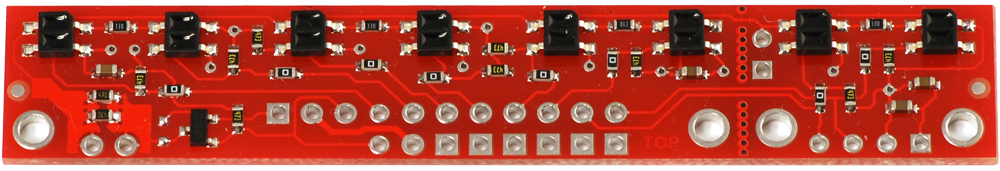
\includegraphics[width=1\textwidth]{QTR-8A.jpg}\par
\quelle\url{https://tinyurl.com/QTR8A-front}

\subsection{Verwendete Libraries}
\paragraph{Pololu QTR Reflectance Sensors}

\bibliographystyle{plain}
\bibliography{literatur}
\end{document}
